%//==============================--@--==============================//%
\label{sec:SistemasDis}
\subsection[6.1 Problemas Representativos de PDE's]{$\rightarrow$ Problemas Representativos de PDE's}
Considere um troço de autoestrada em que se assumem verdadeiras as seguintes hipóteses:

\begin{itemize}
    \item[\ding{43}] Os veículos só podem entrar no início do troço e sair no final do troço.
    \item[\ding{43}] Os veículos não podem sair nem entrar ao longo do troço.
    \item[\ding{43}] Supõe-se que os veículos são suficientemente numerosos para que a densidade de tráfego (número de veículos por unidade de comprimento) seja uma variável contínua.
    \item[\ding{43}] No troço, todos os veículos deslocam-se sempre com uma velocidade constante
\end{itemize}

\noindent Seja $x$ a posição medida em Km a partir do início do troço e $\rho (x,t)$ a densidade de
tráfego (\textit{vehicle density}) no ponto de abcissa $x$, no instante $t$. Na prática, o que se mede é o fluxo de
tráfego $q(x,t)$ , dado pelo número de veículos por unidade de tempo que passam no
ponto de abcissa $x$ no instante $t$.

%//==============================--@--==============================//%

\subsubsection*{$\blacktriangle$ Sejam dois pontos de abcissas $\mathbf{x_2 > x_1}$ . Mostre que a densidade e o fluxo de
tráfego estão relacionados por:}

$$
\frac{\mathrm{d}}{\mathrm{d}t}\int_{x_1}^{x_2}\rho (x,t)dx = q(x_1,t) - q(x_2,t)
$$

\mdfsetup{linewidth=2pt}
\begin{mdframed}
    \noindent $\pmb{\rightarrow}$ \textbf{\textit{Densidade de tráfego (Vehicle density)}:}
     \textit{``The number of vehicles in a unit length of the road at time $t$ and position x. \textbf{A quantity that is easily recorded by observation of traffic flow along a road} is the flux of vehicles $q(x_i,t)$, defined as the number of vehicles that at time $t$ pass a given point with coordinate $x$ in a unit of time.''}
\end{mdframed}

\noindent O número de veículos num dado troço de autoestrada, caracterizado por dois pontos fixos $x_1$ e $x_2$ (onde $x_2$ > $x_1$), pode ser revisto como a diferença entre o fluxo de tráfego de entrada ($x_1$) e de saída ($x_2$) ( já que \textit{``Os veículos só podem entrar no início do troço e sair no final do troço.'')}:

$$
    \textbf{nº de veículos} = q(x_1,t) - q(x_2,t)
$$

\noindent A densidade de veículos no troço é a diferença de densidades entre o seu ponto inicial e final:

$$
    \rho(\Delta x, t) = \rho(x_2, t) - \rho(x_1, t) = \int_{x_1}^{x_2}\rho (x,t)dx
$$

\noindent Subsequentemente, trivialmente se reconhece que densidade de tráfego está subjugada à variação do número de veículos dentro do troço. A \textit{rate of change} da densidade tráfego entre os dois pontos (caracterizada pela derivada em ordem ao tempo do integral supramencionado) pode então ser relacionada com a diferença de fluxos de entrada e saída, tal como explicitado no enunciado.

%//==============================--@--==============================//%
\clearpage
\subsubsection*{$\blacktriangle$ Deduza uma equação às derivadas parciais para $\rho(x,t)$}

É possível obter um modelo simplificado do sistema fazendo um balanço de densidade da tráfego num troço da autoestrada de comprimento $\Delta x$ durante um intervalo $\Delta t$.

\vspace{-0.75em}
\begin{figure}[H]
    \centering
    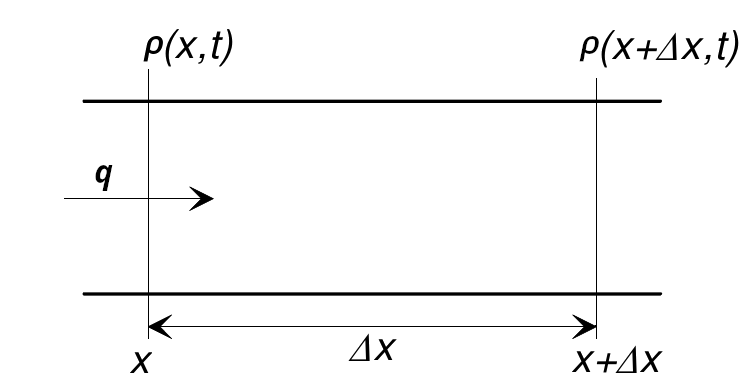
\includegraphics[width = 0.5\linewidth]{img/applied-dif-equ/fluxo-veiculo.png}
    \caption{Vizualização do balanço de densidade para um dado troço de autoestrada}
    \label{fig:fluxoV}
\end{figure}
\vspace{-1.5em}
$$
    \Delta x (\rho(x, t + \Delta t) - \rho(x, t)) = \Delta t (q(x,t) - q(x + \Delta x,t))
$$

\noindent Como $q = \text{v}\rho$ onde v é uma velocidade constante, é possível admitir que:
$$
    \Delta x (\rho(x, t + \Delta t) - \rho(x, t)) = \Delta t \cdot \text{v}(\rho(x,t) - \rho(x + \Delta x,t))
$$

\noindent Dividindo cada parcela da expressão por $\Delta x\Delta t$ e supondo que $\Delta x \to 0$ e $\Delta t \to 0$ obtém-se o modelo na forma de uma equação às derivadas parciais:% amo-te muito :3

$$
    \frac{\partial}{\partial t}\rho(x,t) = -\text{v}\frac{\partial}{\partial x}\rho(x,t)
$$

%//==============================--@--==============================//%
\subsubsection*{$\blacktriangle$ Por substituição na equação e verificação das condições iniciais, mostre que a
solução da equação deduzida é:}
$$
    \rho(x,t) = F(x - \text{v}t)
$$
\textbf{Em que $F(x) = \rho(x,0)$ é a densidade inicial de tráfego.}

\mdfsetup{linewidth=2pt}
\begin{mdframed}
    \noindent $\pmb{\rightarrow}$ Seguindo o método das características para PDE's quasilineares, a solução da equação pode ser vista como o deslocamento de veículos ao longo de um troço de autoestrada:

    $$
       \rho(x,t) = F\left(x - \int_{t_0}^{t}\text{v}\, dt, t_0\right) = 0
    $$
\end{mdframed}

\noindent Consequentemente, podemos provar a veracidade da solução através do uso da condição inicial:

$$
    \rho(x,0) = F\left(x - \int_{0}^{0}\text{v}\, dt, 0\right) = F(x)
$$

%//==============================--@--==============================//%
\clearpage
\subsubsection*{$\blacktriangle$ Mostre que ao longo das retas definidas no plano $[x,t]$ por $\frac{dx}{dt} = \text{v}$ a densidade
de tráfego é constante. Escreva a solução que dá $x$ como função de $t$
para estas rectas (denominadas rectas características. A partir daqui demonstre
a solução da equação às derivadas parciais dada na alínea anterior.}

Avaliando a \textit{rate of change} da densidade de tráfego ao longo do troço:
$$
    \frac{d}{d t}\rho(x,t) = \frac{\partial}{\partial t}\rho(x,t) + \frac{\partial}{\partial x}\rho(x,t)\cdot \frac{dx}{dt}
$$
Facilmente se depreende que os dois termos da parcela direita da equação se anulam:
$$
    \frac{d}{d t}\rho(x,t) = -\text{v}\frac{\partial}{\partial x}\rho(x,t) + \text{v}\frac{\partial}{\partial x}\rho(x,t) = 0
$$
\noindent Se a derivada total em ordem ao tempo (\textit{rate of change}) é nula, então não ocorrem variações ao longo do tempo e a densidade de tráfego é constante. Recorrendo agora à solução obtida na alínea anterior, o mesmo resultado é evidente:
$$
    \frac{d}{d t}\rho(x,t) = \frac{d}{d t}F(x - t) = F(x - \text{v}t)\frac{d}{d t} (x - \text{v}t) = F(x - \text{v}t)(\text{v} - \text{v}) = 0
$$
\noindent\textbf{A densidade de tráfego é constante} $\pmb{\rightarrow}$ A densidade de veículos no troço de autoestrada ao longo do tempo, para cada ponto de deslocamento é sempre a mesma.

%//==============================--@--==============================//%
\subsubsection*{$\blacktriangle$ Considere um troço de autoestrada com 20km e que a velocidade de
circulação é de 120km. Suponha que a densidade inicial de tráfego é definida por:}
\vspace{-1em}
$$
    \rho(x,0) = \begin{cases}
                    25 & 0 \le x \le 2\\
                    0  & x\notin [0,2]\\
                \end{cases}
$$
\noindent\textbf{Represente graficamente a densidade de tráfego em função do tempo no final
do troço. Suporte o seu resultado num desenho tridimensional no espaço}
\begin{itemize}
    \item[$\rightarrow$] A velocidade de circulação é constante, logo, a densidade de tráfego sofre um deslocamento linear para a direita ao longo do tempo.
    \item[$\rightarrow$] A densidade de tráfego não sofre alterações ao longo do troço de autoestrada, logo, a densidade de tráfego é idêntica à inicial para todos os pontos do troço.
\end{itemize}

\noindent O desenho tridimensional terá a seguinte forma:

\begin{figure}[H]
    \centering
    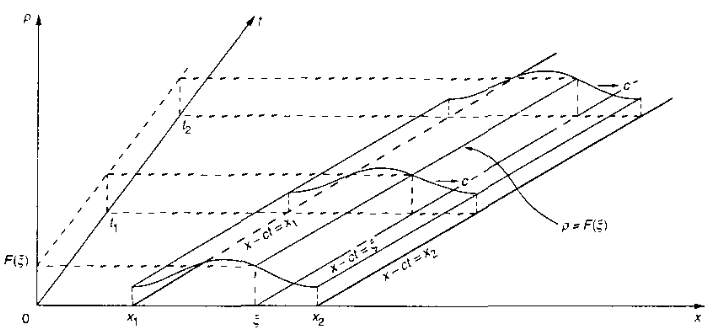
\includegraphics[width = 0.8\linewidth]{img/applied-dif-equ/plot3d.png}
    \caption{Solução geral do problema: $x_1 = 0$ e $p(x,0)$ igual à do enunciado.}
    \label{fig:3dplot}
\end{figure}

%//==============================--@--==============================//%